% Figure 1 - spoof-detector v0.2.1 pipeline block diagram.
% Standalone TikZ source. Compile with: pdflatex fig01_pipeline_block_diagram.tex
%
% Conventions:
%   - Muted academic palette: navy primary, gold accent, neutral grey blocks.
%   - MiniFASNet block: gold accent border to convey "strong per-frame discriminator".
%   - Peak-sensitive verdict block: largest, navy-filled terminal block (headline novelty).
%   - Portrait orientation (taller than wide) for single-column paper template.
\documentclass[border=8pt]{standalone}
\usepackage{amsmath}
\usepackage{tikz}
\usetikzlibrary{positioning,shapes.geometric,arrows.meta,fit,backgrounds,calc}

% --- palette ----------------------------------------------------------------
\definecolor{paperNavy}{HTML}{1F3A5F}
\definecolor{paperGold}{HTML}{B8860B}
\definecolor{paperBlock}{HTML}{F4F4EF}
\definecolor{paperRule}{HTML}{4A4A4A}
\definecolor{paperGroup}{HTML}{E9ECEF}
\definecolor{paperEmph}{HTML}{FFF8E1}

\begin{document}
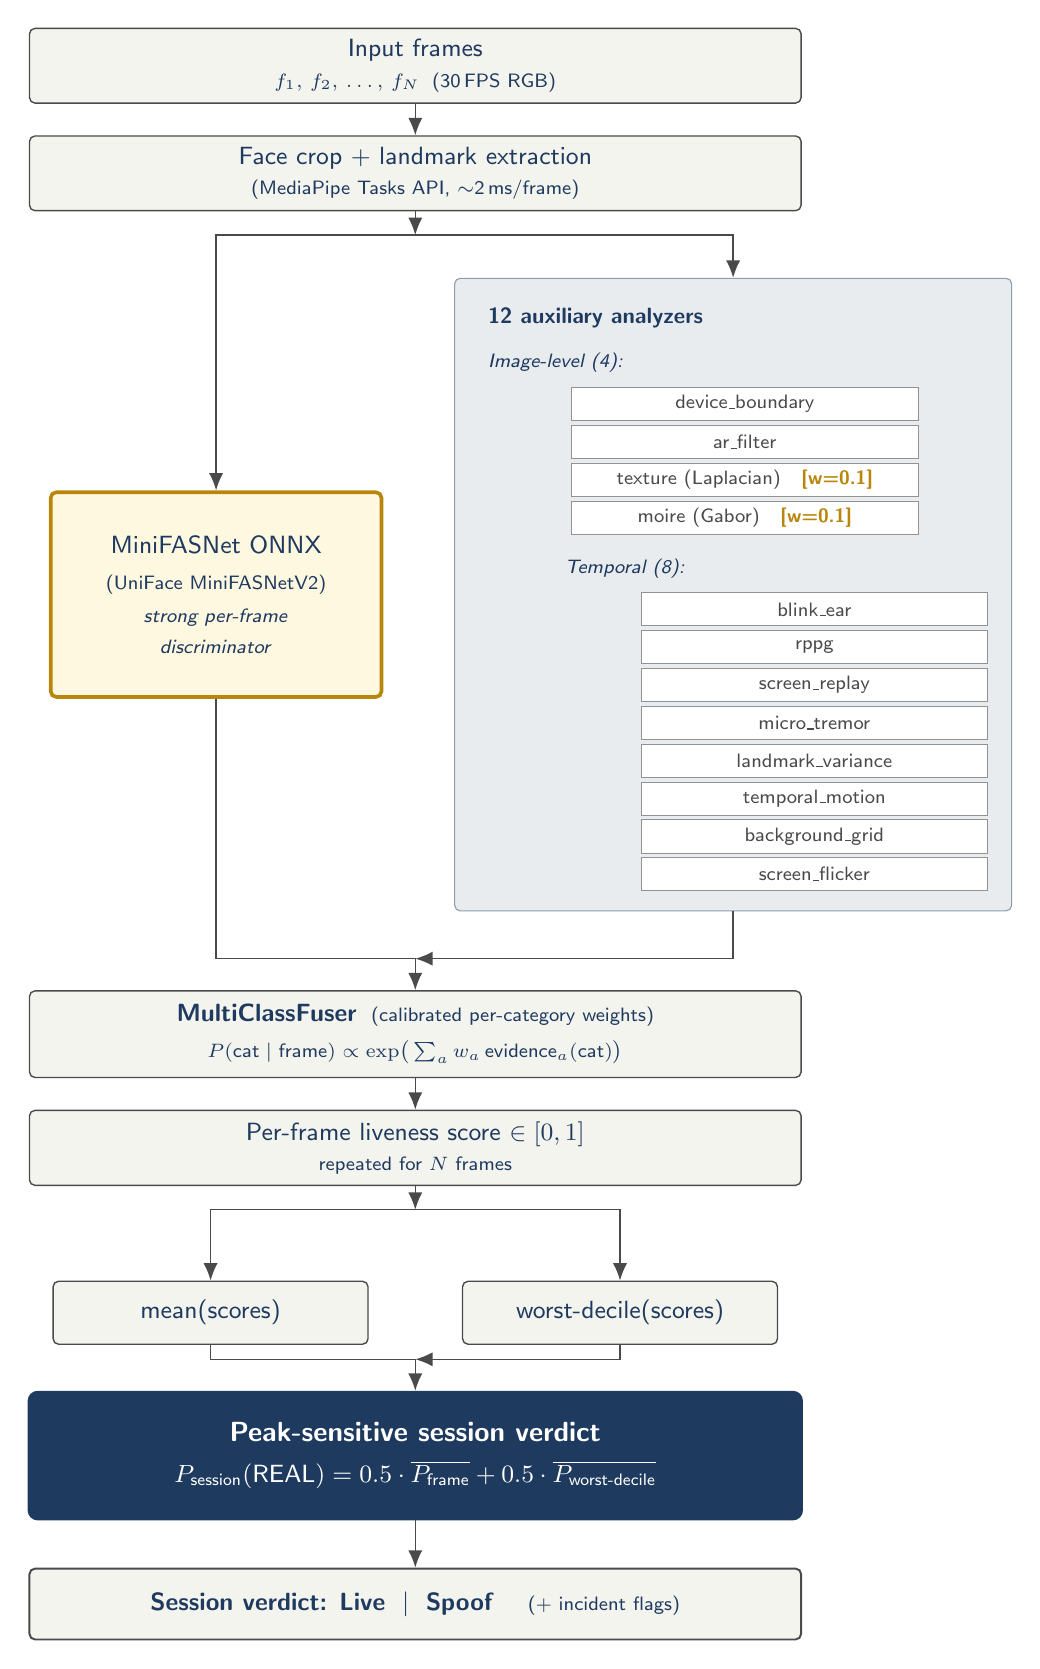
\begin{tikzpicture}[
    font=\sffamily\small,
    >={Latex[length=2.2mm,width=1.8mm]},
    every node/.style={align=center},
    block/.style={
        rectangle, rounded corners=2pt, draw=paperRule, line width=0.5pt,
        fill=paperBlock, minimum height=8mm, inner sep=4pt, text=paperNavy
    },
    emphblock/.style={
        rectangle, rounded corners=2pt, draw=paperGold, line width=1.3pt,
        fill=paperEmph, minimum height=9mm, inner sep=5pt, text=paperNavy
    },
    verdictblock/.style={
        rectangle, rounded corners=3pt, draw=paperNavy, line width=1.3pt,
        fill=paperNavy, text=white, minimum height=16mm, minimum width=98mm,
        inner sep=6pt, font=\sffamily\bfseries
    },
    terminalblock/.style={
        rectangle, rounded corners=2pt, draw=paperRule, line width=0.7pt,
        fill=paperBlock, minimum height=9mm, inner sep=5pt, text=paperNavy,
        font=\sffamily\bfseries\small
    },
    analyzer/.style={
        rectangle, draw=paperRule!60, line width=0.3pt, fill=white,
        minimum height=4.2mm, minimum width=44mm, inner sep=1.5pt,
        font=\sffamily\scriptsize, text=paperRule
    },
    grouphdr/.style={
        font=\sffamily\scriptsize\itshape, text=paperNavy, anchor=north west
    },
    arr/.style={->, draw=paperRule, line width=0.55pt},
    node distance=4mm and 5mm
]

% --- input ------------------------------------------------------------------
\node[block, minimum width=98mm] (input)
    {Input frames\\ \scriptsize $f_1,\,f_2,\,\ldots,\,f_N$ \;(30\,FPS RGB)};

\node[block, below=of input, minimum width=98mm] (facecrop)
    {Face crop $+$ landmark extraction\\ \scriptsize (MediaPipe Tasks API, $\sim$2\,ms/frame)};

% --- analyzer bank: MiniFASNet (left) + 12 auxiliary analyzers (right) -----
% We build the auxiliary column first, then place MiniFASNet to align vertically.

% Anchor the aux column at a known coordinate below facecrop.
\coordinate (auxanchor) at ($(facecrop.south) + (8mm,-11mm)$);

\node[font=\sffamily\bfseries\footnotesize, anchor=north west, text=paperNavy]
    (auxhdr) at (auxanchor) {12 auxiliary analyzers};

\node[grouphdr] (imghdr) at ($(auxhdr.south west) + (0,-0.8mm)$)
    {Image-level (4):};
\node[analyzer, below=0.6mm of imghdr.south, anchor=north west, xshift=2mm]
    (a1) {device\_boundary};
\node[analyzer, below=0.5mm of a1.south, anchor=north]
    (a2) {ar\_filter};
\node[analyzer, below=0.5mm of a2.south, anchor=north]
    (a3) {texture (Laplacian)\quad\textcolor{paperGold}{\bfseries [w=0.1]}};
\node[analyzer, below=0.5mm of a3.south, anchor=north]
    (a4) {moire (Gabor)\quad\textcolor{paperGold}{\bfseries [w=0.1]}};

\node[grouphdr] (temphdr) at ($(a4.south west) + (-2mm,-1.8mm)$)
    {Temporal (8):};
\node[analyzer, below=0.6mm of temphdr.south, anchor=north west, xshift=2mm]
    (t1) {blink\_ear};
\node[analyzer, below=0.5mm of t1.south, anchor=north] (t2) {rppg};
\node[analyzer, below=0.5mm of t2.south, anchor=north] (t3) {screen\_replay};
\node[analyzer, below=0.5mm of t3.south, anchor=north] (t4) {micro\_tremor};
\node[analyzer, below=0.5mm of t4.south, anchor=north] (t5) {landmark\_variance};
\node[analyzer, below=0.5mm of t5.south, anchor=north] (t6) {temporal\_motion};
\node[analyzer, below=0.5mm of t6.south, anchor=north] (t7) {background\_grid};
\node[analyzer, below=0.5mm of t7.south, anchor=north] (t8) {screen\_flicker};

% Group frame around the aux column - drawn behind via background layer.
\begin{scope}[on background layer]
    \node[rectangle, rounded corners=2pt, draw=paperNavy!50, line width=0.4pt,
          fill=paperGroup, inner xsep=3mm, inner ysep=2.5mm,
          fit=(auxhdr)(a1)(a4)(temphdr)(t1)(t8)] (auxbox) {};
\end{scope}

% MiniFASNet: positioned to the left of auxbox, vertically centered on it.
\node[emphblock, minimum width=42mm, minimum height=26mm, align=center,
      anchor=east] (minifas) at ($(auxbox.west) + (-9mm,0)$)
    {MiniFASNet ONNX\\[2pt]
     \scriptsize (UniFace MiniFASNetV2)\\[1pt]
     \scriptsize \textit{strong per-frame}\\
     \scriptsize \textit{discriminator}};

% --- fuser ------------------------------------------------------------------
% Anchor below the lower of (minifas.south, auxbox.south), centered horizontally.
\coordinate (postaux) at ($(auxbox.south) + (0,-10mm)$);
\node[block, minimum width=98mm, minimum height=11mm,
      anchor=north] (fuser) at ($(input.south |- postaux)$)
    {\textbf{MultiClassFuser}\;\;\scriptsize (calibrated per-category weights)\\[2pt]
     \scriptsize $P(\text{cat}\mid \text{frame}) \propto \exp\!\big(\sum_{a} w_a\,\text{evidence}_a(\text{cat})\big)$};

\node[block, below=of fuser, minimum width=98mm] (perframe)
    {Per-frame liveness score $\in [0,1]$\\
     \scriptsize repeated for $N$ frames};

% --- session aggregator (two summary statistics) ---------------------------
\node[block, below=12mm of perframe.south, xshift=-26mm,
      minimum width=40mm] (mean) {mean(scores)};
\node[block, below=12mm of perframe.south, xshift=26mm,
      minimum width=40mm] (worst) {worst-decile(scores)};

% --- verdict (terminal, emphasized) ----------------------------------------
\node[verdictblock, below=12mm of perframe.south, yshift=-14mm] (verdict)
    {Peak-sensitive session verdict\\[3pt]
     \normalfont\sffamily\small $P_\text{session}(\text{REAL})
        = 0.5\cdot\overline{P_\text{frame}}
        + 0.5\cdot\overline{P_\text{worst-decile}}$};

\node[terminalblock, below=6mm of verdict, minimum width=98mm] (final)
    {Session verdict: \textsc{Live} \;$\mid$\; \textsc{Spoof} \;\;
     \scriptsize\mdseries{(+ incident flags)}};

% --- arrows -----------------------------------------------------------------
\draw[arr] (input) -- (facecrop);

% facecrop -> minifas + auxbox (fan-out)
\coordinate (fanout1) at ($(facecrop.south) + (0,-3mm)$);
\draw[arr] (facecrop.south) -- (fanout1);
\draw[arr] (fanout1) -| (minifas.north);
\draw[arr] (fanout1) -| (auxbox.north);

% minifas + auxbox -> fuser (fan-in)
\coordinate (fanin1) at ($(fuser.north) + (0,4mm)$);
\draw[arr] (minifas.south) |- (fanin1) -- (fuser.north);
\draw[arr] (auxbox.south)  |- (fanin1);

\draw[arr] (fuser) -- (perframe);

% perframe -> mean + worst (fan-out)
\coordinate (fanout2) at ($(perframe.south) + (0,-3mm)$);
\draw[arr] (perframe.south) -- (fanout2);
\draw[arr] (fanout2) -| (mean.north);
\draw[arr] (fanout2) -| (worst.north);

% mean + worst -> verdict (fan-in)
\coordinate (fanin2) at ($(verdict.north) + (0,4mm)$);
\draw[arr] (mean.south)  |- (fanin2) -- (verdict.north);
\draw[arr] (worst.south) |- (fanin2);

\draw[arr] (verdict) -- (final);

\end{tikzpicture}
\end{document}
